%%%%%%%%%%%%%%%%%%%%%%%%%%%%%%%%%%%% Chapter 

\chapter{Les Résultats} 	
\label{Chapter3} 		

%%%%%%%%%%%%%%%%%%%%%%%%%%%%%%%%%%%%%%%%%%%%%%%%%%%%%%%%%%%%%%%%%%%%%%%%%%%%%%%%
%%%%%%%%%%%%%%%%%%%%%%%%%%%%%%%%%%%% SECTION 1 %%%%%%%%%%%%%%%%%%%%%%%%%%%%%%%%%
%%%%%%%%%%%%%%%%%%%%%%%%%%%%%%%%%%%%%%%%%%%%%%%%%%%%%%%%%%%%%%%%%%%%%%%%%%%%%%%%

\section{2D - résultats par alpha}
\label{sec:Ch3.1}

\begin{figure}[H]
    \centering
    \begin{subfigure}[b]{\textwidth}
        \centering
        \resizebox{\textwidth}{!}{%
            \begin{tabular}{|c|c|c|c|c|c|c|c|c|c|c|c|c|c|c|c|c|c|c|c|c|c|}
                \hline
                \textbf{$\alpha$} & 0 & 1 & 2 & 3 & 4 & 5 & 6 & 7 & 8 & 9 & 10 & 11 & 12 & 13 & 14 & 15 & 16 & 17 & 18 & 19 & 20 \\ \hline
                \textbf{$\text{diamètre}_{\text{opti}}$} & 0.040 & 0.091 & 0.098 & 0.098 & 0.10  & 0.10  & 0.10  & 0.10  & 0.095 & 0.089 & 0.079 & 0.061 & 0.040 & 0.040 & 0.040 & 0.040 & 0.040 & 0.040 & 0.040 & 0.040 & 0.040 \\ \hline
                \textbf{$\text{cambrure}_{\text{opti}}$} & 0.20 & 0.00 & 0.00 & 0.01 & 0.04 & 0.06 & 0.068 & 0.074 & 0.078 & 0.082 & 0.086 & 0.093 & 0.103 & 0.105 & 0.107 & 0.109 & 0.111 & 0.113 & 0.115 & 0.118 & 0.121 \\ \hline
            \end{tabular}
        }
        \caption{Valeurs optimales pour chaque alpha}
        \label{fig:table}
    \end{subfigure}
    
    \vspace{10mm} % Ajout d'espace entre le tableau et l'image

    \begin{subfigure}[b]{\textwidth}
        \centering
        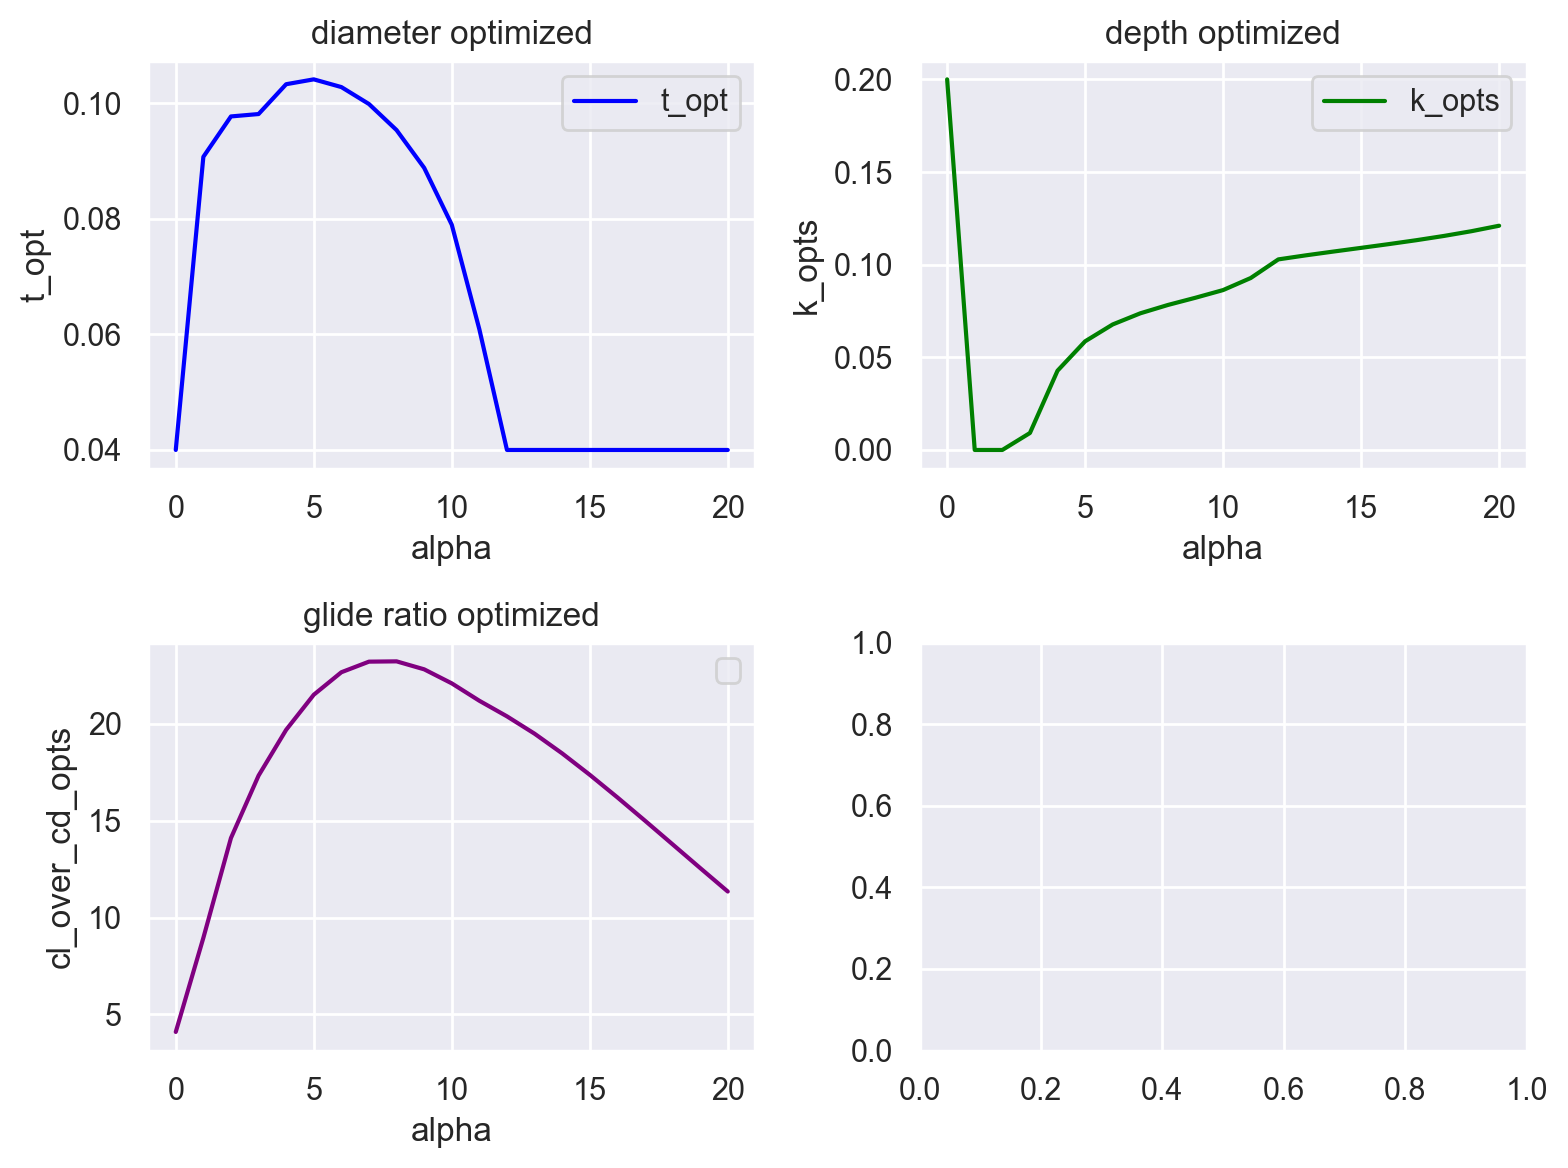
\includegraphics[width=0.6\textwidth]{Pics/03 - Les résultats/résultats pas alpha 2D.png}
        \caption{Tracer de t et k optimaux pour chaque alpha}
        \label{fig:graph}
    \end{subfigure}
    \caption{Résultats 2D optimaux (finesse) de diamètre et cambrure par alpha}
    \label{fig:opti alpha 2d}
\end{figure}



\textbf{On observe que pour les grands angles le diamètre optimal tend à être le plus petit possible. La cambrure optimale augmente avec $\alpha$. Les résultats sont cohérents en ordre de grandeur}

%%%%%%%%%%%%%%%%%%%%%%%%%%%%%%%%%%%%%%%%%%%%%%%%%%%%%%%%%%%%%%%%%%%%%%%%%%%%%%%%
%%%%%%%%%%%%%%%%%%%%%%%%%%%%%%%%%%%% SECTION 2 %%%%%%%%%%%%%%%%%%%%%%%%%%%%%%%%%
%%%%%%%%%%%%%%%%%%%%%%%%%%%%%%%%%%%%%%%%%%%%%%%%%%%%%%%%%%%%%%%%%%%%%%%%%%%%%%%%

\section{2D - résultats moyennes pondérées par Gaussienne}
\label{sec:Ch3.2}


\begin{figure}[h!]
    \centering
    \begin{subfigure}[b]{0.45\textwidth}
        \centering
        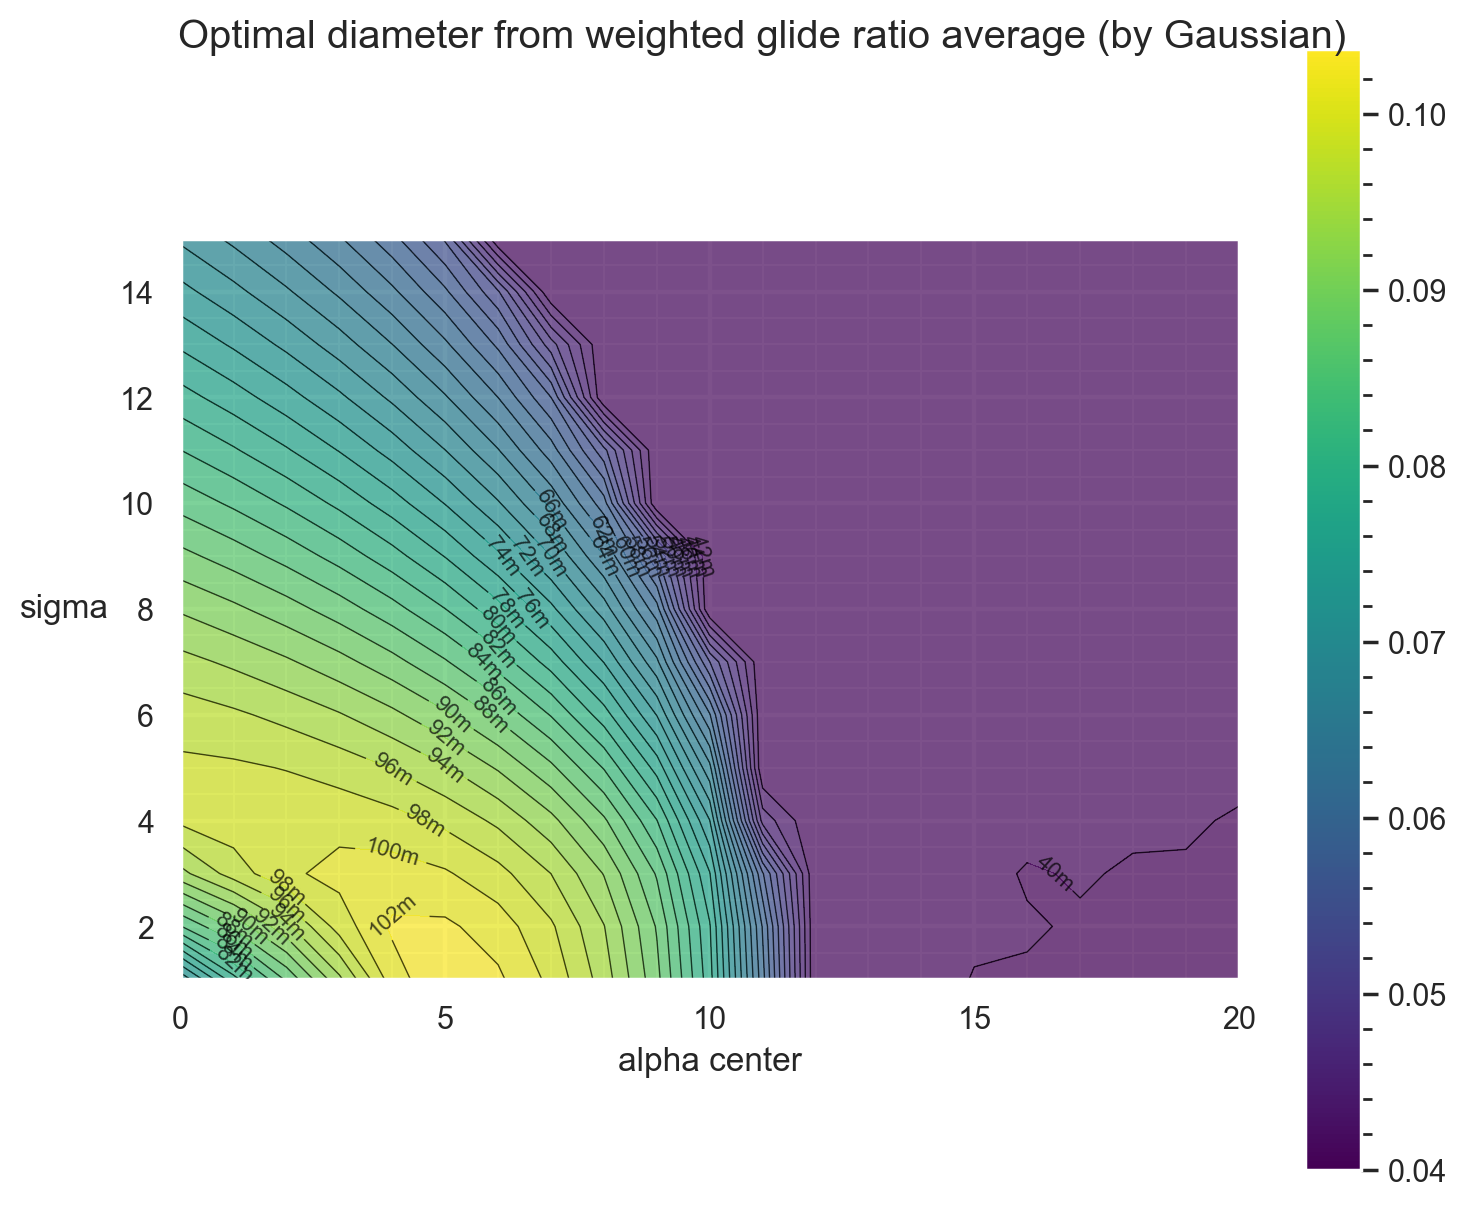
\includegraphics[width=\linewidth]{Pics/03 - Les résultats/diametre gaussian 2d.png}
        \caption{diamètre selon les paramètres de la Gaussienne}
        \label{fig:diametre gaussien 2d}
    \end{subfigure}
    \hfill 
    \begin{subfigure}[b]{0.45\textwidth}
        \centering
        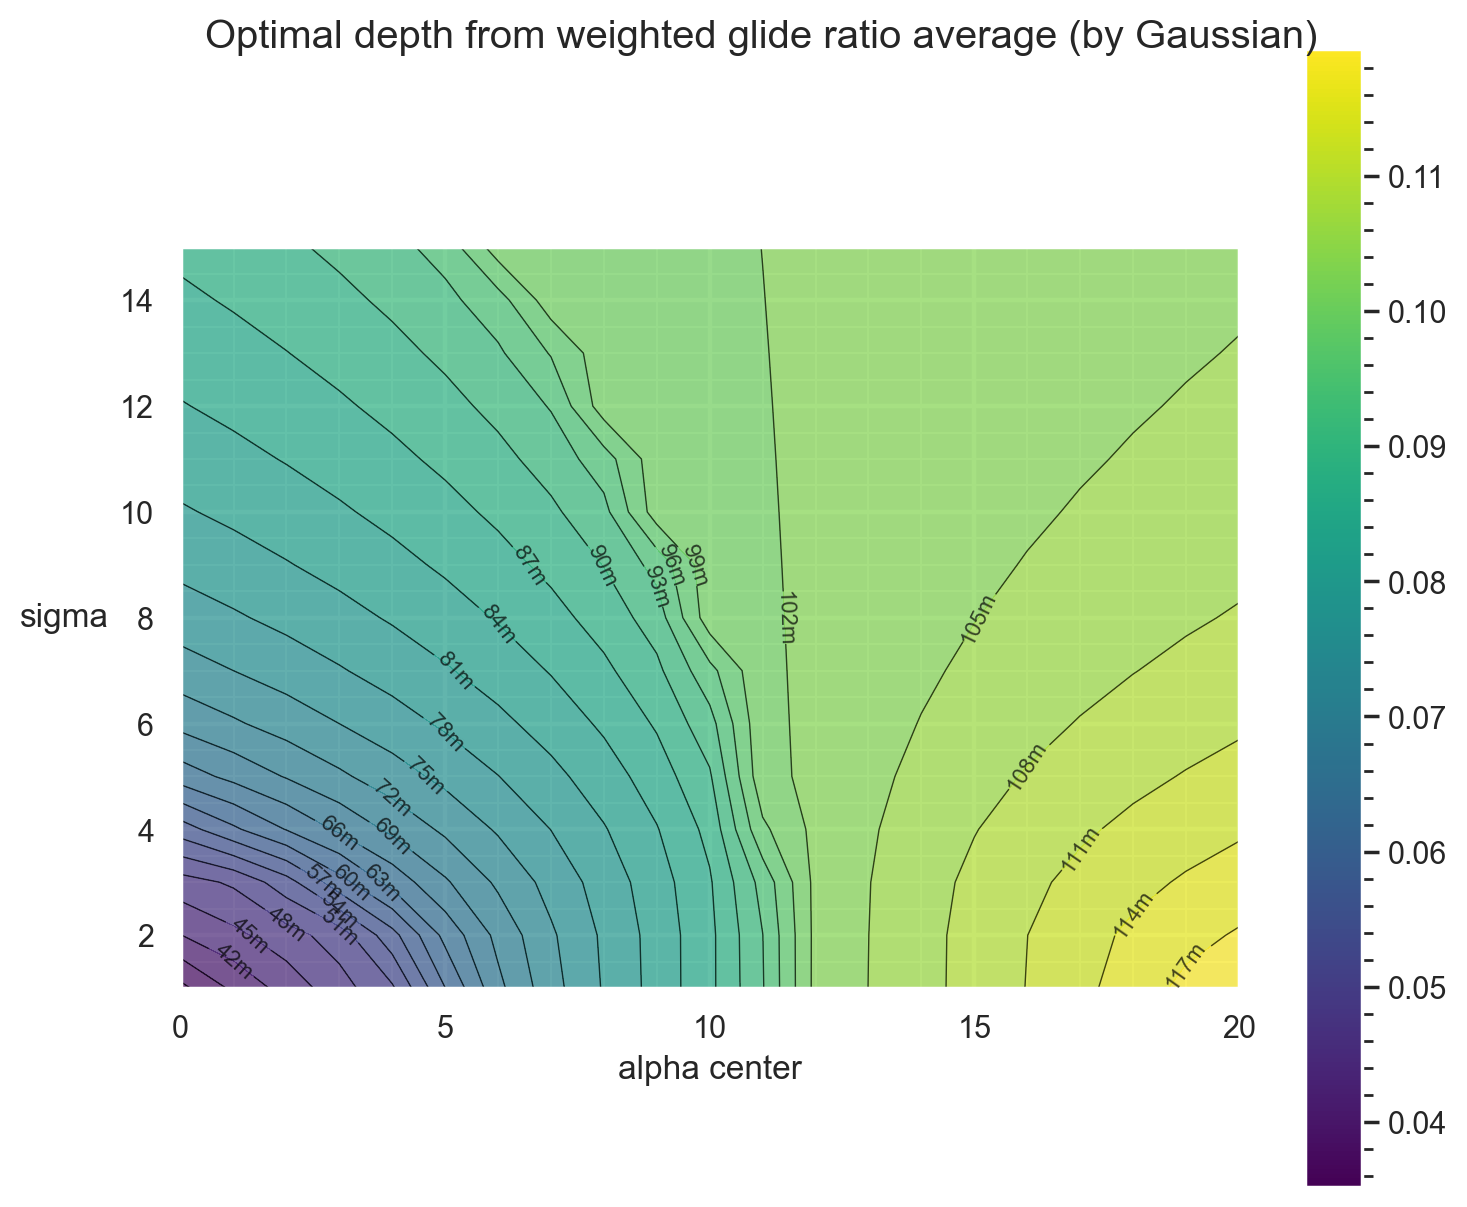
\includegraphics[width=\linewidth]{Pics/03 - Les résultats/depth gaussian 2d.png}
        \caption{cambrure selon les paramètres de la Gaussienne}
        \label{fig:cambrure gaussien 2d}
    \end{subfigure}
    \caption{Sensibilité des résultats 2D en fonction de l'écart-type $\sigma$ et de la valeur centrale $\alpha_{center}$ de la Gaussienne}
    \label{fig:gaussian sensibility 2d}
\end{figure}

\textbf{Pour $\sigma$ proche de zéro (écart-type "très petit"), les résultats convergent vers ceux de la partie précédente. }\\

\textbf{Le diamètre optimal} augmente avec $\alpha_{center}$ (jusqu'à environ 5°) puis diminue avec $\alpha_{center}$ pour des $\sigma$ inférieurs à 4. Augmenter $\sigma$ (i.e. "prendre davantage d'angles en considération") tend à diminuer le diamètre pour $\alpha_{center}$ plus grand que 5. Le diamètre optimal sature à sa valeurs minimale au delà de 12°. \\

\textbf{La cambrure optimale} augmente avec $\alpha$. Elle augmente avec $\sigma$ pour alpha inférieur à 12° et diminue avec $\sigma$ pour alpha plus grand.
*
%%%%%%%%%%%%%%%%%%%%%%%%%%%%%%%%%%%%%%%%%%%%%%%%%%%%%%%%%%%%%%%%%%%%%%%%%%%%%%%%
%%%%%%%%%%%%%%%%%%%%%%%%%%%%%%%%%%%% SECTION 3 %%%%%%%%%%%%%%%%%%%%%%%%%%%%%%%%%
%%%%%%%%%%%%%%%%%%%%%%%%%%%%%%%%%%%%%%%%%%%%%%%%%%%%%%%%%%%%%%%%%%%%%%%%%%%%%%%%

\section{3D - résultats par alpha}
\label{sec:Ch3.3}

Le tableau suivant présente les résultats obtenu avec la VSM (3D). Les nombres de ribs saturés en diamètre/cambrure sont, pour chaque alpha, les nombre de ribs qui ne pouvaient pas atteindre la valeurs objective (Valeurs initiale + delta) et qui donc sont "saturés" à la valeurs minimal ( $\frac{Diamètre}{2}$ pour la cambrure et 0.04 pour le diamètre).\\

A noter que les ribs initialement à faible diamètre (relatif) sont ceux du bord d'attaque, et que les profils les moins cambré sont aux tips; en témoigne les valeurs initiales de t et k présentés en II.B..

\begin{figure}[H]
    \centering
    % Tableau (lignes et colonnes inversées)
    \begin{subfigure}[b]{\textwidth}
        \centering
        \resizebox{\textwidth}{!}{%
            \begin{tabular}{|c|c|c|c|c|c|c|c|c|c|c|c|c|c|c|c|c|c|c|c|c|c|}
                \hline
                \textbf{$\alpha$} & 0 & 1 & 2 & 3 & 4 & 5 & 6 & 7 & 8 & 9 & 10 & 11 & 12 & 13 & 14 & 15 & 16 & 17 & 18 & 19 & 20 \\ \hline
                \textbf{\parbox{2.2cm}{\centering $\delta$diamètre}} 
                    & -0.02 & -0.007 & -0.007 & -0.007 & -0.007 & -0.007 & -0.007 & -0.007 & -0.02 & -0.02 & -0.02 & 0.033 & 0.033 & 0.033 & 0.02 & 0.02 & 0.02 & 0.02 & -0.007 & -0.007 & -0.007 \\ \hline
                \textbf{\parbox{2.5cm}{\centering Nombre ribs saturés en diamètre}} 
                    & 10 & 0 & 0 & 0 & 0 & 0 & 0 & 0 & 0 & 0 & 0 & 0 & 0 & 0 & 0 & 0 & 0 & 0 & 0 & 0 & 0 \\ \hline
                \textbf{\parbox{2.2cm}{\centering $\delta$cambrure}} 
                    & -0.1 & -0.1 & -0.1 & -0.1 & -0.1 & -0.1 & -0.1 & -0.1 & -0.1 & -0.1 & -0.1 & -0.033 & -0.033 & -0.1 & -0.1 & -0.1 & -0.1 & -0.1 & 0.1 & 0.1 & 0.1 \\ \hline
                \textbf{\parbox{2.5cm}{\centering Nombre ribs saturés en cambrure}} 
                    & 20 & 20 & 20 & 20 & 20 & 20 & 20 & 20 & 20 & 20 & 20 & 12 & 12 & 4 & 4 & 4 & 4 & 4 & 0 & 0 & 0 \\ \hline
            \end{tabular}
        }
        \caption{Valeurs optimales pour chaque alpha}
        \label{fig:table}
    \end{subfigure}
    
    \vspace{10mm} % Ajout d'espace entre le tableau et l'image
    
    % Image
    \begin{subfigure}[b]{\textwidth}
        \centering
        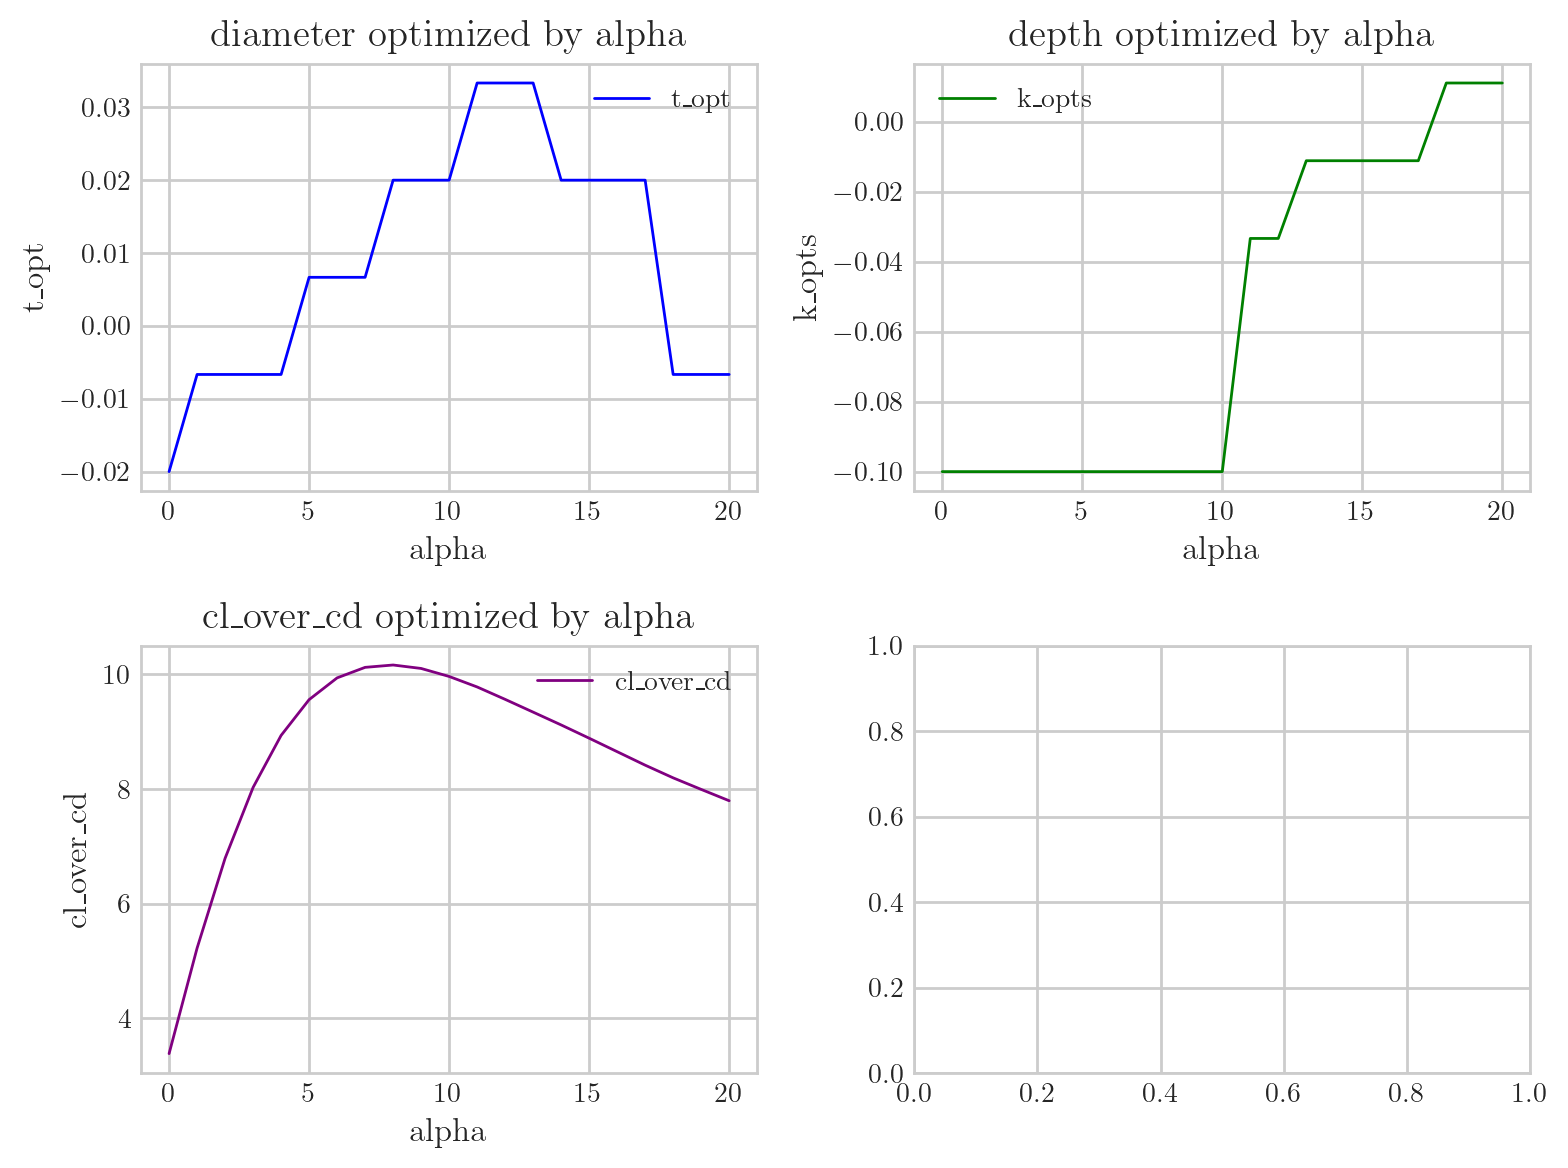
\includegraphics[width=0.7\textwidth]{Pics/03 - Les résultats/résultats pas alpha 3D.png}
        \caption{Tracer de t et k optimaux pour chaque alpha}
        \label{fig:graph}
    \end{subfigure}
    
    % Légende globale
    \caption{Résultats 3D optimaux (finesse) de diamètre et cambrure par alpha}
    \label{fig:opti_alpha_3d}
\end{figure}



\textbf{On observe que le diamètre optimal augmente avec $\alpha$ jusqu'à 13° puis diminue. La cambrure sature à sa valeurs minimale en dessous de 10° puis augumente avec $\alpha$ }

%%%%%%%%%%%%%%%%%%%%%%%%%%%%%%%%%%%%%%%%%%%%%%%%%%%%%%%%%%%%%%%%%%%%%%%%%%%%%%%%
%%%%%%%%%%%%%%%%%%%%%%%%%%%%%%%%%%%% SECTION 4 %%%%%%%%%%%%%%%%%%%%%%%%%%%%%%%%%
%%%%%%%%%%%%%%%%%%%%%%%%%%%%%%%%%%%%%%%%%%%%%%%%%%%%%%%%%%%%%%%%%%%%%%%%%%%%%%%%

\section{3D - résultats moyennes pondérées par Gaussienne}
\label{sec:Ch3.4}

\begin{figure}[H]
    \centering
    \begin{subfigure}[b]{0.45\textwidth}
        \centering
        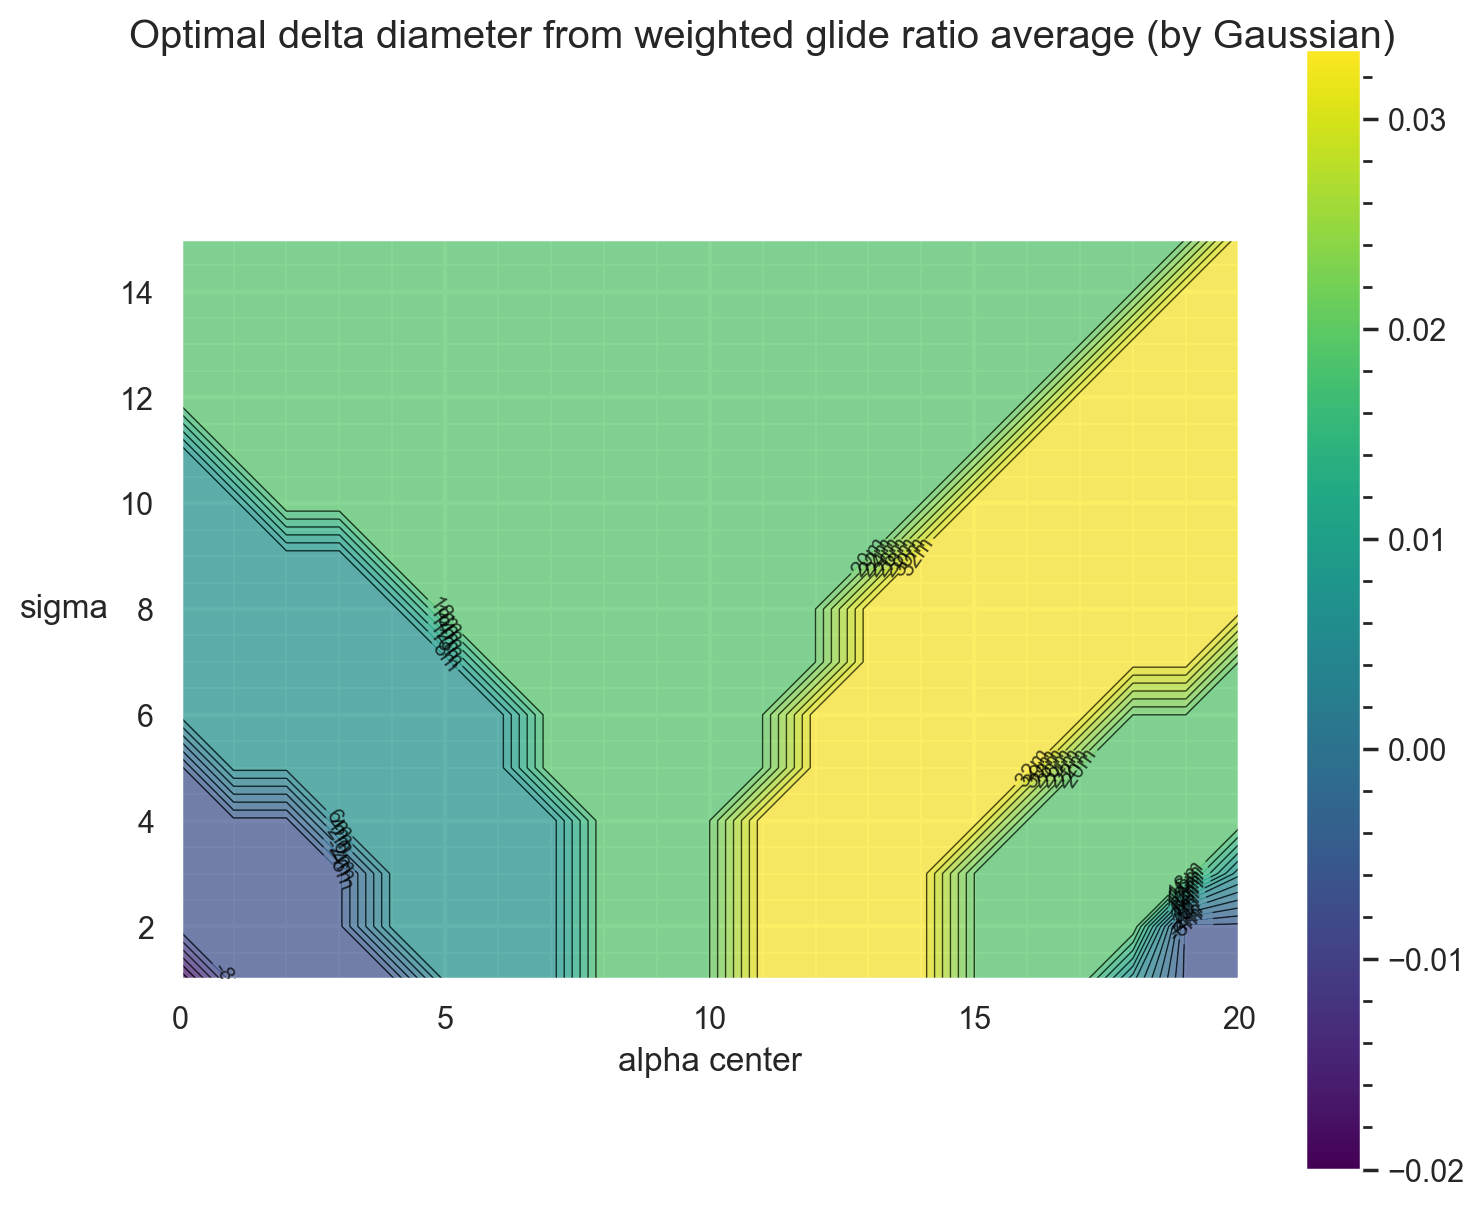
\includegraphics[width=\linewidth]{Pics/03 - Les résultats/diametre gaussian.png}
        \caption{$\delta$ diamètre selon les paramètres de la Gaussienne}
        \label{fig:diametre gaussien}
    \end{subfigure}
    \hfill
    \begin{subfigure}[b]{0.45\textwidth}
        \centering
        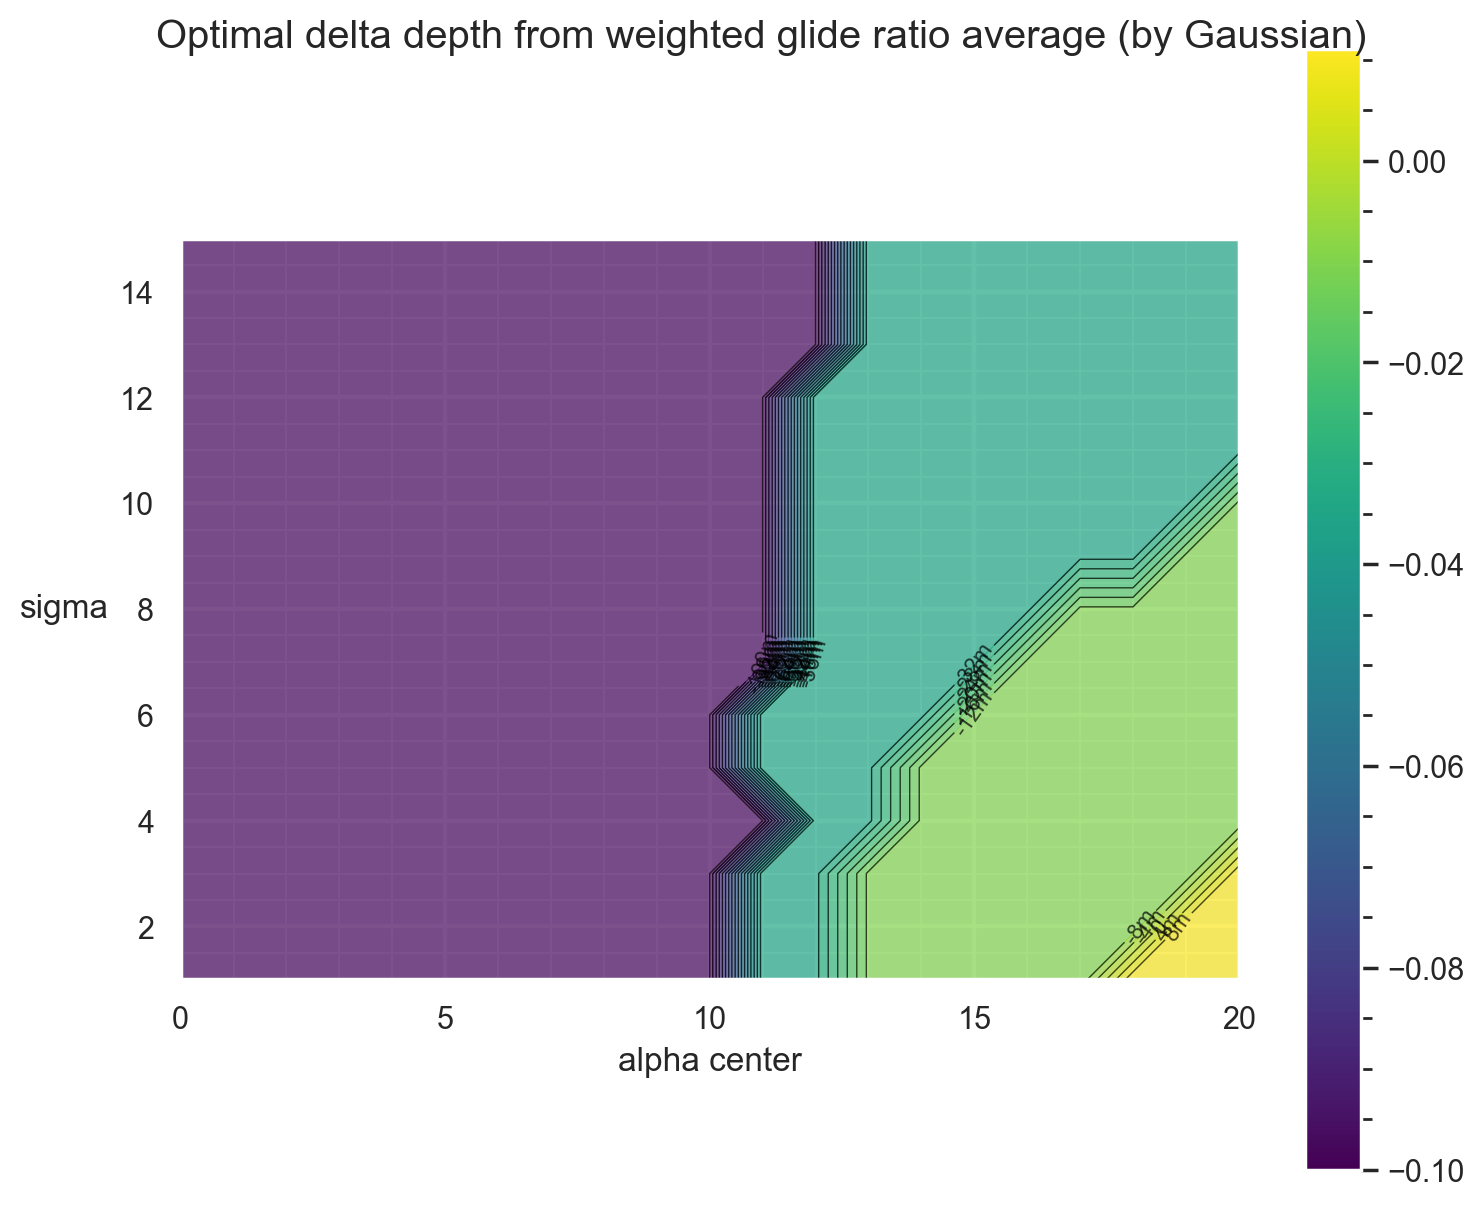
\includegraphics[width=\linewidth]{Pics/03 - Les résultats/depth gaussian.png}
        \caption{$\delta$ cambrure selon les paramètres de la Gaussienne}
        \label{fig:cambrure gaussien}
    \end{subfigure}
    \caption{Sensibilité des résultats 3D en fonction de l'écart-type $\sigma$ et de la valeur centrale $\alpha_{center}$ de la Gaussienne}
    \label{fig:gaussian sensibility}
\end{figure}


Sur la figure \ref{fig:gaussian sensibility} (comme sur la figure \ref{fig:gaussian sensibility 2d}), on rappelle que $\sigma$ proche de zéro signife un écart-type quasi nul, i.e. on retrouve les mêmes résultats que sur la figure \ref{fig:opti_alpha_3d}. A l'inverse, $\sigma$ grand signifie qu'on augmente l'influence des angles autours de $\alpha_{center}$ sur la moyenne pondérée; fonction objective de l'optimisation. \\

\textbf{ On observe qu'augmenter $\sigma$ diminue la cambrure optimale. Le comportement est identique pour le diamètre si $\alpha_{center}$ est supérieur à 15°; le comportement inverse en dessous de 15°}
    
%%%%%%%%%%%%%%%%%%%%%%%%%%%%%%%%%%%%%%%%%%%%%%%%%%%%%%%%%%%%%%%%%%%%%%%%%%%%%%%%
%%%%%%%%%%%%%%%%%%%%%%%%%%%%%%%%%%%% SECTION 5 %%%%%%%%%%%%%%%%%%%%%%%%%%%%%%%%%
%%%%%%%%%%%%%%%%%%%%%%%%%%%%%%%%%%%%%%%%%%%%%%%%%%%%%%%%%%%%%%%%%%%%%%%%%%%%%%%%

\section{3D - Exemple d'exploitation de résultats 3D}
\label{sec:Ch3.5}

Avec une Gaussienne de paramètres \textbf{center = 7° et sigma = 8}, les valeurs qui maximisent la fonction objective (moyenne pondérée de finesse aérodynamique) sont :
\begin{itemize}
    \item $\delta diameter$ : 0.02
    \item $\delta depth$ : -0.1
\end{itemize}
\smallskip

\textbf{Les valeurs de diamètre et cambrure optimaux ainsi obtenus en 3D sont : 
}
\begin{itemize}
    \item t : 0.090 0.086 0.085 0.083 0.081 0.080 0.080  0.080 0.080 0.080 0.080  0.080 0.080 0.080 0.080 0.081 0.083 0.085 0.087 0.090
    \item k : 0.045 0.043 0.043 0.041 0.040 0.040 0.040  0.040 0.040 0.040 0.040 0.040 0.040 0.040  0.040 0.040 0.041 0.043 0.043 0.045
\end{itemize}
\smallskip

\textbf{A comparer avec les valeurs initiales :}
\begin{itemize}
    \item t : 0.07 0.067 0.065 0.063 0.061 0.06 0.06  0.06 0.06 0.06  0.06  0.06 0.06 0.06  0.06 0.061 0.063 0.065 0.067 0.07
    \item k : 0.034 0.05 0.0645 0.0686 0.072 0.075 0.08 0.08 0.08 0.08 0.08 0.08 0.08 0.08 0.075 0.072 0.0686 0.0645 0.05 0.034
\end{itemize}

\textbf{On note donc une tendance (en 3D) à augumenter le diamètre du BA et diminuer la cambrure du kite. }
